\section{Imagen-Video}
\label{sec:imagen_video}

\begin{figure}
    \centering
    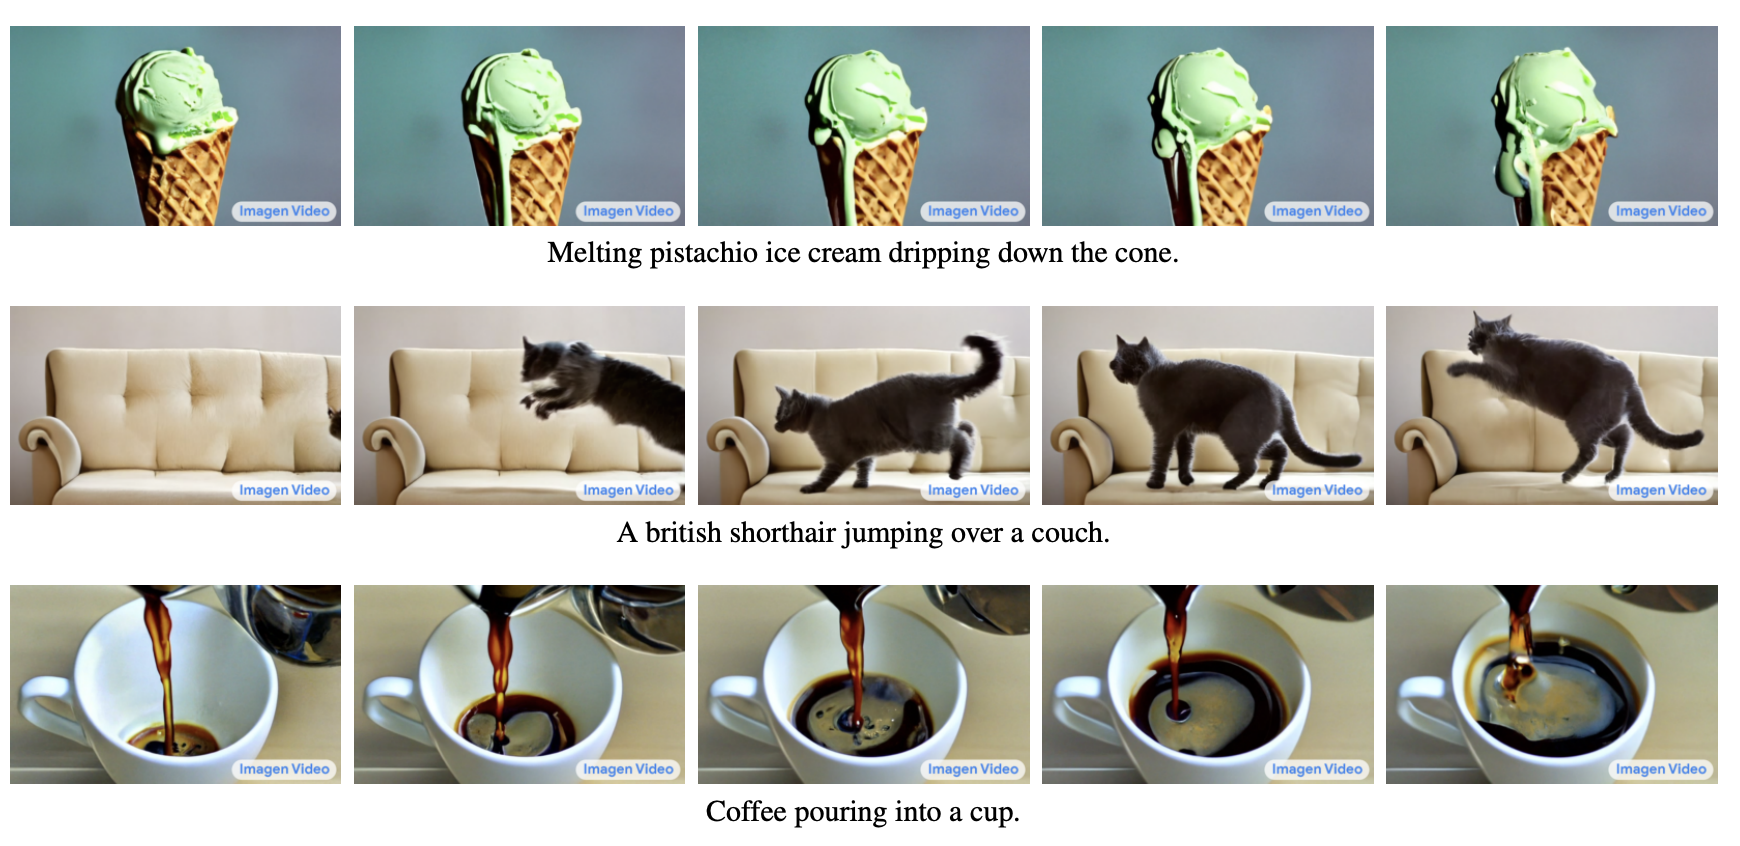
\includegraphics[width=1\textwidth]{images/video_synthesis/imagen_video.png}
    \caption{Imagen-Video video samples examples.}
\end{figure}

\begin{figure}
    \centering
    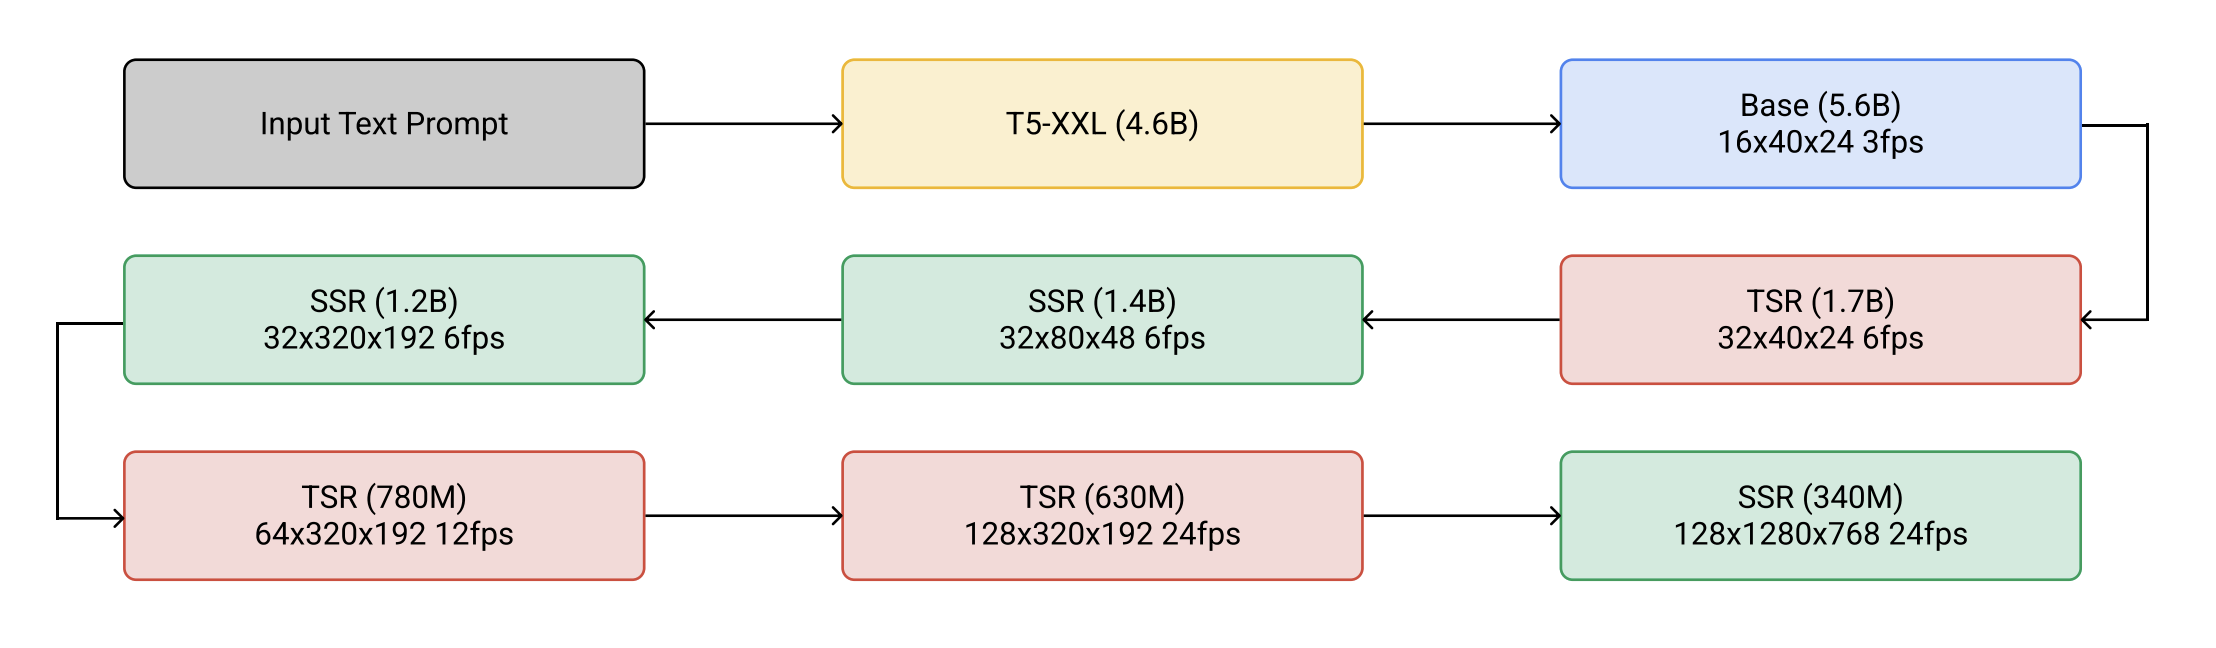
\includegraphics[width=1\textwidth]{images/imagen_video/pipeline.png}
    \caption{Imagen-Video cascading pipeline. The text embeddings are injected to all models in the pipeline (its not shown).}
    \label{fig:imagen_video_pipeline}
\end{figure}

Imagen-Video by Google \cite{imagen_video} is a text-to-video cascading diffusion model, based on previous work: Imagen (section \ref{sec:imagen}). It builds on the cascaded nature of Imagen. In total, Imagen-Video has 7 sub-models in a cascading pipeline (figure \ref{fig:imagen_video_pipeline}). Imagen-Video generates high definition $1280\times 768$ videos @ 24 fps, for 5.3 seconds. A big downside of Imagen-Video compared to Video-LDM is that Imagen-Video works in the pixel-space, whereas Video-LDM works in latent space. In addition, Imagen-Video is a much larger model and uses more resources than Video-LDM, however Google is able to achieve good results through massive training scaling.

Like Imagen, Imagen-Video uses the same large frozen text-encoder T5-XXL (section \ref{subsec:t5})in its pipeline.

The benefit of cascading pipeline is the ability to independently train each model, allowing the parallel training of all 7 models. Another benefit is the ability to use the super-resolution models, which are general purpose video super-resolution models, independently on downstream tasks.


\begin{figure}
    \centering
    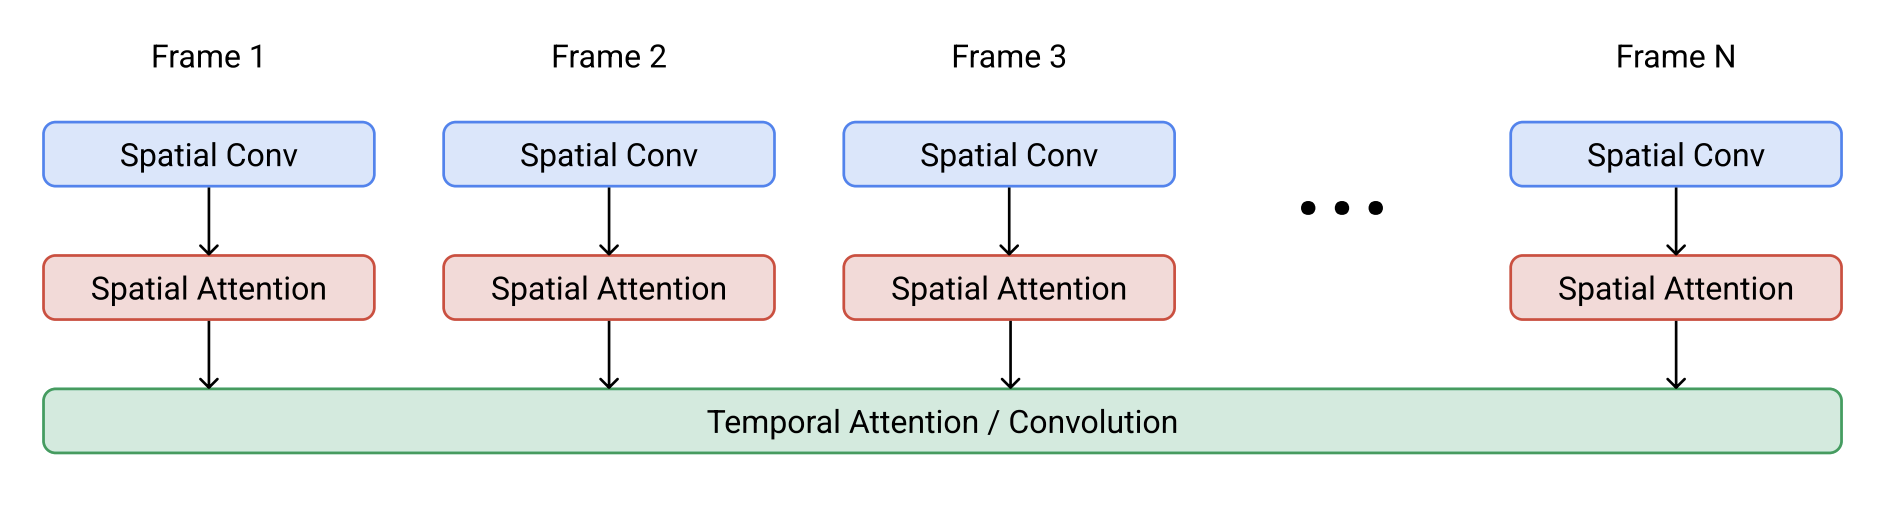
\includegraphics[width=1\textwidth]{images/imagen_video/video_u_net.png}
    \caption{Video U-Net block \cite{video_diffusion_models} used by Imagen-Video. Each frame independently processed by spatial convolution and spatial attention, while a collection of frames are processed by temporal attention and convolution.}
    \label{fig:imagen_video_video_unet}
\end{figure}


Imagen Video also builds on the work of \textbf{Video U-Net} \cite{video_diffusion_models}, which generalizes the 2D diffusion model architecture to 3D in space-time by using temporal attention and 3D convolution layers to capture dependencies between video frames. See figure \ref{fig:imagen_video_video_unet}.

In Imagen-Video paper, the researchers write that due to the safety and ethical challenges in training the Imagen-Video model, \textbf{they decided not to release the model to the public} (closed source).

One of the contribution of the paper is that they successfully transferred multiple methods from the image domain to video, such as \textbf{v-parameterization \cite{v_prediction}, classifier-free guidance and conditioning augmentation} \cite{cascaded_diffusion_models}. They also found out that \textbf{progressive distillation} \cite{v_prediction} \cite{meng2023distillation} is a valuable technique for speeding up video sampling.














\subsection{Architecture}

Imagen Video has 1 frozen text encoder, 1 base video diffusion model, three SSR (spatial super-resolution) models, and three TSR (temporal super-resolution) models (totaling 7 video diffusion models). Each of the denoising diffusion models $\hat{x_\theta}$ operate on multiple video frames simultaneously.

Whereas typically diffusion models for image generation use a 2D U-Net architecture (spatial attention and convolution), \textbf{Video U-Net} block used by Imagen-Video (figure \ref{fig:imagen_video_video_unet}) generalizes the U-Net to 3D space-time by using temporal attention and convolution to capture dependencies between video frames.

Imagen-Video pipeline is compromised of the following model types:

\begin{itemize}
    \item \textbf{T5-XXL:} As we discussed before, T5-XXL is a text-to-text transformer used to encode (text encoder) the text prompts to embeddings (tokens). These tokens condition all of the 7 diffusion models (not only the base model as shown in figure \ref{fig:imagen_video_video_unet}).
    \item \textbf{Base:} The base diffusion model generate low FPS low resolution video clip, it uses temporal attention.
    \item \textbf{SSR:} The SSR model is a spatial super-resolution (SSR) model that increases the resolution of the input image to higher spatial resolution. Unlike the base model, it uses temporal convolution instead of temporal attention. Like SR3, we first apply bilinear or bicubic interpolation to increase the resolution, then we remove noise (add details) by first concatenating noise $y_t$ to the upsampled image $x$ and then use the U-Net denoising network to learn to denoise the image.
    \item \textbf{TSR:} The TSR model is a temporal super-resolution (TSR) model that increases the temporal resolution of the input video (increases frame count). To achieve this, they \textbf{fill in intermediate frames between input frames}. Unlike the base model, it uses temporal convolution instead of temporal attention.
\end{itemize}


\textbf{Temporal Attention v.s. Temporal Convolution}: The base diffusion model uses temporal attention because they want it to learn to model long term temporal dependencies, whereas the SSR and TSR models use temporal convolution instead, which maintains local temporal consistency. \textbf{Temporal convolution reduces memory and computation costs over temporal attention}, which is critical for the SSR and TSR models, which are applied to high-resolution high-fps videos. This is why temporal attention is used at the beginning of the cascading pipeline.

\textbf{Spatial attention at the beginning of the pipeline}: The base model and the first two SSR models have spatial attention in addition to spatial convolution, because it improves sample fidelity, and the attention mechanism is used in the beginning of the pipeline which requires less compute resources than at the end of the pipeline. For example, the last SSR model in the pipeline is a fully convolutional model.

\textbf{Number of parameters}: Imagen Video consists of 11.6 billion parameters. Each of the model's parameters count is shown in figure \ref{fig:imagen_video_pipeline}.

\textbf{Classifier-free guidance}: CFG is also used in Imagen-Video. They found that it helps the model generate high fidelity samples with respect to the text prompts. Higher guidance weights lead the model to focus more on the text prompt conditioning.

\textbf{Oscillating guidance}: Similar to Imagen, when the guidance weight is too large, the possible range of values of predicted noise is beyond $[-1, 1]$, which causes train-test mismatch. This leads to significant artifacts in the generated videos. \textbf{Dynamic thresholding}, as described in Imagen section, helps to prevent this issue, which dynamically clip the image to the chosen threshold followed by scaling by $s$: \texttt{np.clip(x, -s, s) / s}. However, constant high guidance weight leads to saturation artifacts, especially at high resolutions. The researchers didn't find dynamic thresholding sufficient, therefor they experimented with letting the guidance weight \textbf{oscillate between high and low values} for a certain number of sampling steps. They apply this oscillating dynamic threshold only to the base and first SR models. The generation starts with a high guidance weight to establish a strong alignment with the prompt, then alternates between high and low weights in subsequent steps.













\subsection{v-prediction}

In a 2022 paper by Google \cite{v_prediction} the research team introduced a fast sampling method called "progressive distillation" for diffusion models. It allows the diffusion model to sample in a fixed amount of model evaluations, instead of thousands (like in DDPM samplers). They presented a way to distill a trained deterministic diffusion sampler (such as \textbf{DDIM} (section \ref{subsec:ddim_sampler}) and appendix \ref{appendix:dm_samplers}) that takes as half as many sampling steps. Each distillation halves the number of required sampling steps.

For example, state-of-the-art samplers that take 8192 steps can be distilled down to as few as 4 steps without significant loss in perceptual quality.

Progressive distillation depends on "v-prediction" (velocity prediction). Instead of predicting the noise in U-Net (called $\epsilon$-prediction), v-prediction focuses on predicting the velocity of the diffusion process, which denotes the rate of change of the image with respect to time.

\begin{figure}
    \centering
    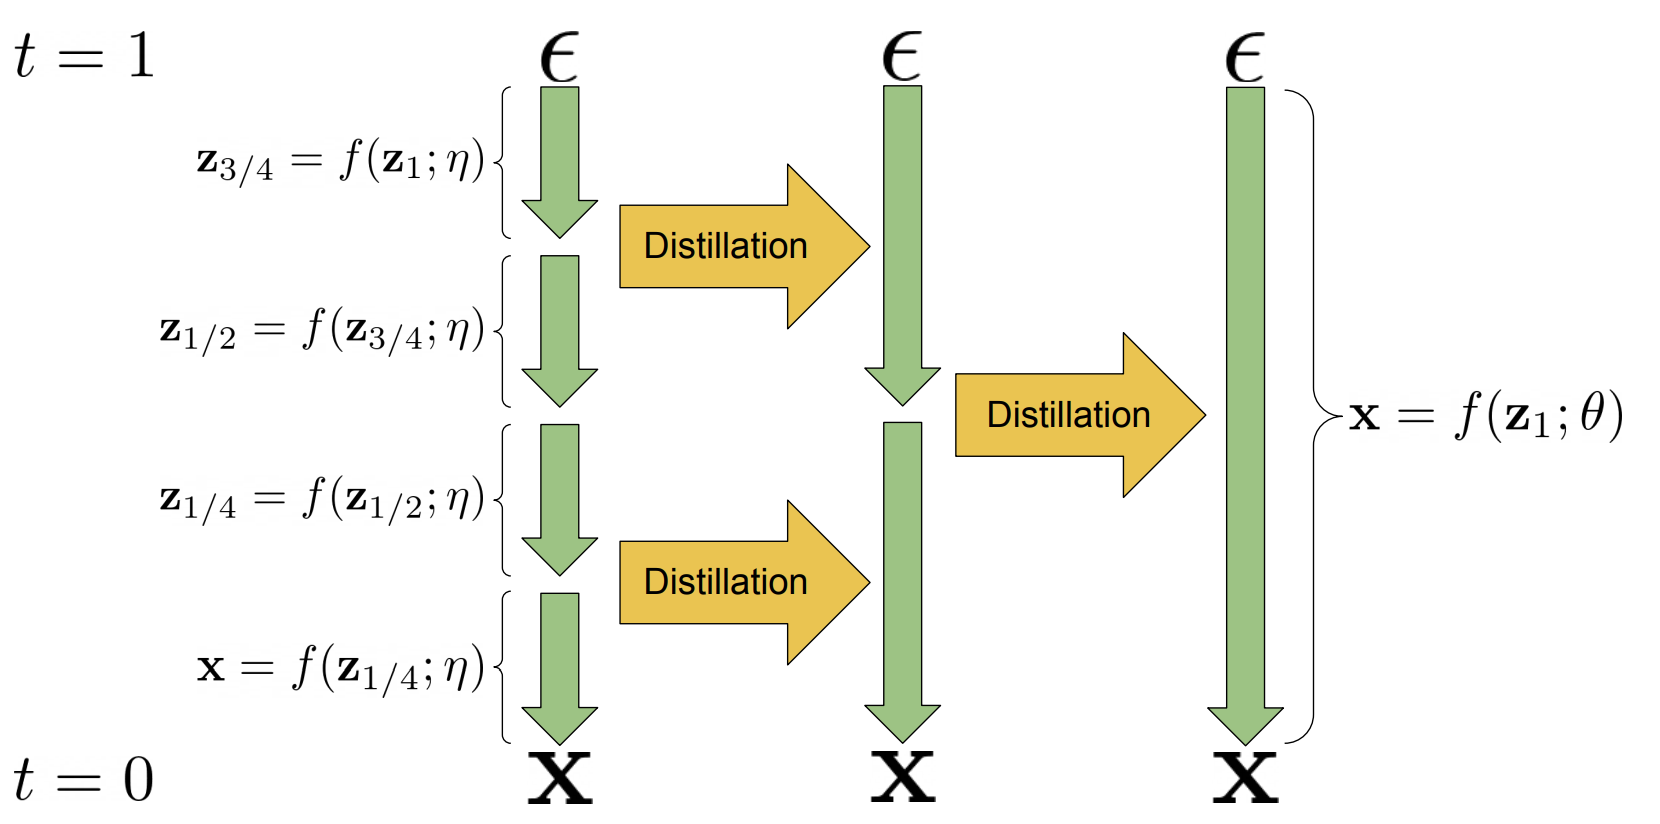
\includegraphics[width=0.6\textwidth]{images/imagen_video/v_prediction.png}
    \caption{v-prediction: A fast sampling method for diffusion models. Instead of taking 4 sampler ($f(z; \eta)$) steps to transform from noise $\epsilon$ to an image $x$, we distilled the model and now it takes a single step.}
    \label{fig:progressive_distillation}
\end{figure}

\begin{figure}
    \centering
    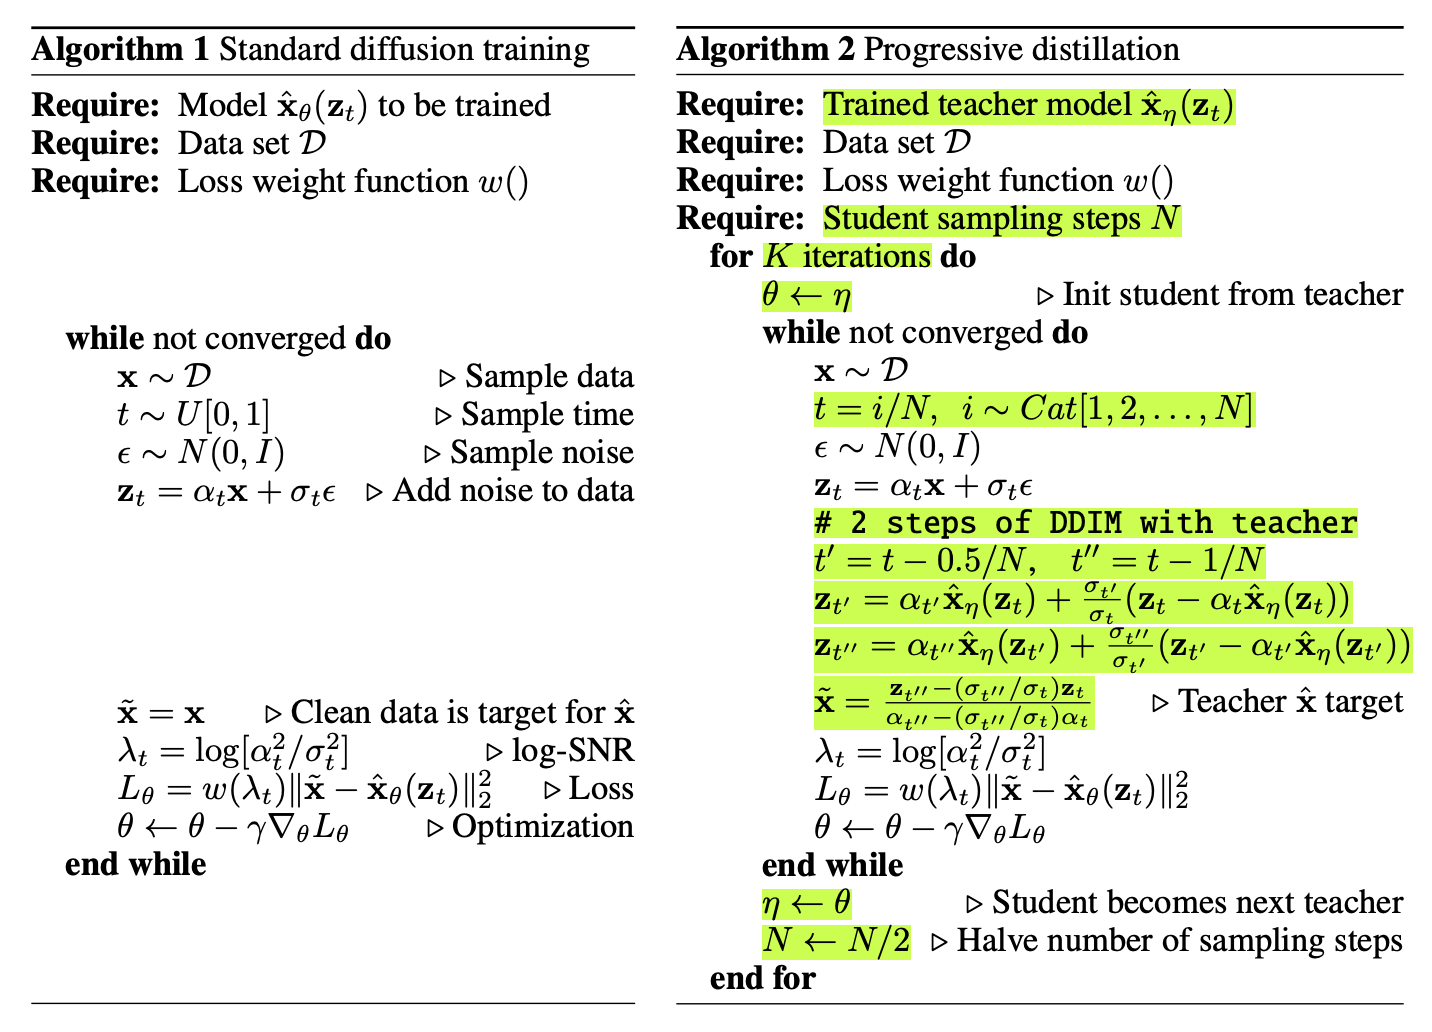
\includegraphics[width=0.7\textwidth]{images/imagen_video/progressive_distillation.png}
    \caption{Progressive distillation algorithm. After the student model (with parameters $\eta$) is distilled to match the output of the teacher model, the teacher model becomes the student model and the process is repeated.}
    \label{fig:progressive_distillation_algorithm}
\end{figure}

This is achieved by creating a sequence of models, where each model ("\textbf{student}") is trained to mimic a previous, slower model ("\textbf{teacher}") that requires more steps to produce a sample. In each distillation step the student model is initialized with the weights of the teacher model; 

The teacher model uses standard sampling approach, such as DDIM, and then the student model learns to approximate this process in fewer steps.

In figure \ref{fig:progressive_distillation_algorithm} the trained teacher model $\hat{x}_{\eta} (z_t)$ is the trained diffusion model $\hat{x}_{\theta} (z_t)$, where $z_t$ is the noisy data (we take training data $\mathcal{D}$ and add noise to it). Now we modify this model and make it sample faster by changing the teacher model to the student model, after we distilled the student model. The student model learns to predict $\tilde{x}$ which is the result of two steps of the teacher model (by using two DDIM steps). This way the student model learns to match the two-step output of the previous (teacher) model in one step.

In the Imagen-Video paper, they used v-prediction parametrization:

\[ v \equiv \alpha_t \epsilon - \sigma_t x \]

After training on $N$ sampling steps, we repeat this process with $N/2$ steps and so on.

\begin{figure}
    \centering
    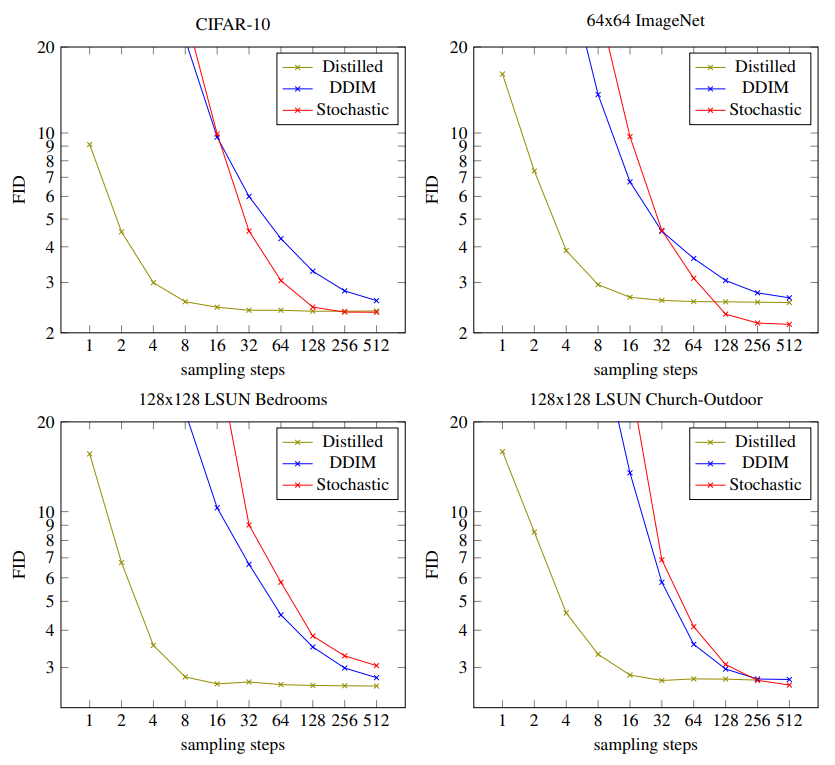
\includegraphics[width=0.7\textwidth]{images/imagen_video/samplers_comparison.png}
    \caption{Comparison of v-prediction sampling to DDIM and stochastic samplers. The distilled model achieves significant lower FID scores with significantly fewer sampling steps (converges faster).}
\end{figure}

The v-prediction parametrization allows progressive distillation across all of the diffusion models in the pipeline, which ultimately allows faster inference. At higher resolutions, v-prediction avoids temporal color shifting artifacts.












\subsection{Noise conditioning augmentation}

Similar to Imagen, Imagen-Video applied noise conditioning augmentation for all the spatial and temporal diffusion models.

In Imagen the researchers used noise conditioning augmentation to \textbf{corrupt low-resolution images}, and the \textbf{SR models would be conditioned on the noise level}. During training, the corruption noise level ("\textbf{augmentation level}") is chosen randomly. This helps the model to generalize better to various noise levels.

This technique is used primarily in cascading pipeline models, such as Imagen and Imagen-Video. It improves the quality and diversity of samples by changing the noise levels at different stages of training, which helps the model generalize better to various noise levels. The model receives conditioning information about the noise level its handling which guides the model to denoise it, similar to how the model receives timestep embeddings $t$ in the diffusion process; its injected in a similar way.

This technique was introduced in a 2021 paper \cite{cascaded_diffusion_models} by Google.











\subsection{Video-image joint training}

Training on both images and videos data allows the model to learn from both types of data, which improves the model's performance in terms of image and video fidelity. In addition, data of text-video pairs is scarce, and it allows \textbf{knowledge transfer from images to videos}. As a result, this join training enables the model to learn to generate different styles of videos.

Imagen-Video follows the same joint training approach as \cite{video_diffusion_models} (a 2022 paper by Google), in which the model is jointly trained from image and video data. During training, \textbf{individual images are treated as a single frame videos}.

To bypass the temporal components on image data during training, they \textbf{apply a mask to the temporal computation paths}. This masking operation causes the model not to apply temporal operations across frames.











\subsection{Progressive distillation with guidance and stochastic samplers}

The researchers in the progressive distillation paper \cite{v_prediction} write why \textbf{$\epsilon$-prediction doesn't work well in distillation}: they say that in distillation we have to work at higher noise levels to the point where the signal-to-noise ratio (SNR) drops down to zero, at which point predicting the noise becomes a lot harder. This is why they turn to $v$-prediction.

An extension of the work of \cite{v_prediction} is the paper \cite{meng2023distillation} by Google Research and Stability AI, which \textbf{extends the distillation to models trained with classifier-free guidance}. This is the first time both the work of distilling models and classifier-free guidance is applied to video domain. As we remember, classifier-free guidance has unconditional prediction and conditional prediction which guides the model with guidance weight of both predictions. The paper also works on distilling the model; the idea is that the teacher model (which is trained with CFG) will take two DDIM steps, and the student model needs to match the teacher output, but instead of doing classifier-free guidance of the student model, the student is \textbf{conditioned on the guidance scale}. In the paper they call the student model a $w$-conditioned model. Conditioning the student model on the guidance weight (incorporated into the diffusion model backbone, similar to how time-step was incorporated in \cite{kingma2021variational}). In the paper \cite{meng2023distillation} they optimize the student model with the following objective:

\begin{equation*}
\mathbb{E}_{w \sim p_w, t \sim U[0, 1], x \sim p_{\text{data}}(x)} 
\left[ 
    \omega(\lambda_t) \left\| 
        \underbrace{\hat{x}_{\eta_1}(z_t, w)}_{\text{student's pred}} - 
        \underbrace{\hat{x}_{\theta}^w(z_t) }_{\text{teacher's pred}}
    \right\|_2^2 
\right]
\end{equation*}

where:

\begin{itemize}
    \item $w$ is the guidance weight and is picked from $p_w$ (which can be fixed or oscillate, but in Imagen-Video they chose to oscillate)
    \item $p_w(w) = U[w_{\text{min}}, w_{\text{max}}]$ is the oscillating guidance weight
    \item $t$ is the diffusion timestep
    \item $x$ is the data (images): $x \sim p_{\text{data}}(x)$
    \item $z_t$ is the noised version of $x$ (noisy image at timestep $t$)
    \item $\lambda_t$ is the guidance scale (not really important)
    \item $\omega(\lambda_t)$ is the weighting function (also not really important)
    \item $\hat{x}_{\eta_1}$ is the student model (which is conditioned on the guidance weight $w$ as input: $\hat{x}_{\eta_1}(z_t, \textcolor{red}{w})$). Also notice the notation: $\hat{x}_{\eta_\mathbf{\textcolor{red}{1}}}$, which means that this is the first distillation iteration.
    \item $\hat{x}_{\theta}^w$ is the teacher model. Notice in the notation, its using the guidance weight in CFG (its not conditioned on it, we apply it): $\hat{x}_{\theta}^\mathbf{\textcolor{red}{w}}(z_t)$.
\end{itemize}

Also notice that the teacher model's parameters ($\eta$) are different to the student model's parameters ($\theta$), since they change at each distillation step (the student is a copy of the teacher but to differentiate between the parameters after the distillation process they chose different notation).



In the paper the mathematical notation for CFG for the teacher's model is:

\[  
    \underbrace{
        \hat{x}_{\theta}^w(z_t) = 
        \underbrace{(1+w) \hat{x}_{c,\theta} (z_t)}_{\text{conditional score}} - 
        \underbrace{w \hat{x}_\theta (z_t)}_{\text{unconditional score}}
    }_{\text{teacher CFG}}
\]

where $c$ is the teacher model's conditioning (for example, text prompt) \footnote{Thanks to \href{https://www.youtube.com/watch?v=ZXuK6IRJlnk}{this youtube tutorial} for explaining both papers}.

After a lot of experiments, at the end, \cite{meng2023distillation} decided to go with a new \textbf{$N$-step stochastic sampler} to sample from the distilled model.

To summarize, Using the work of \cite{meng2023distillation}, Imagen-Video researchers successfully distilled 7 video diffusion models with CFG to just 8 sampling steps without any noticeable loss in perceptual quality in the pipeline.














\subsection{Experiments}

In their experiments, they sampled video clips at 192x320 resolution @ 24 fps for 128 frames (5.3 seconds). They repeat the evaluations over four runs and report the mean and standard error.

\textbf{Datasets}: The researchers used 14 billion video-text pairs and 60 million image-text pairs from internal and public datasets, such as LAION-400M \cite{laion_400m}.

\textbf{Resizing}: They resized images using \textbf{antialiased bilinear resizing} and temporally resize videos by \textbf{skipping frames}.

\textbf{Evaluation}: They used FID on individual video frames, FVD for temporal consistency, and frame-wise CLIP scores for video-text alignment (they take the average across all frames).

\begin{figure}
    \centering
    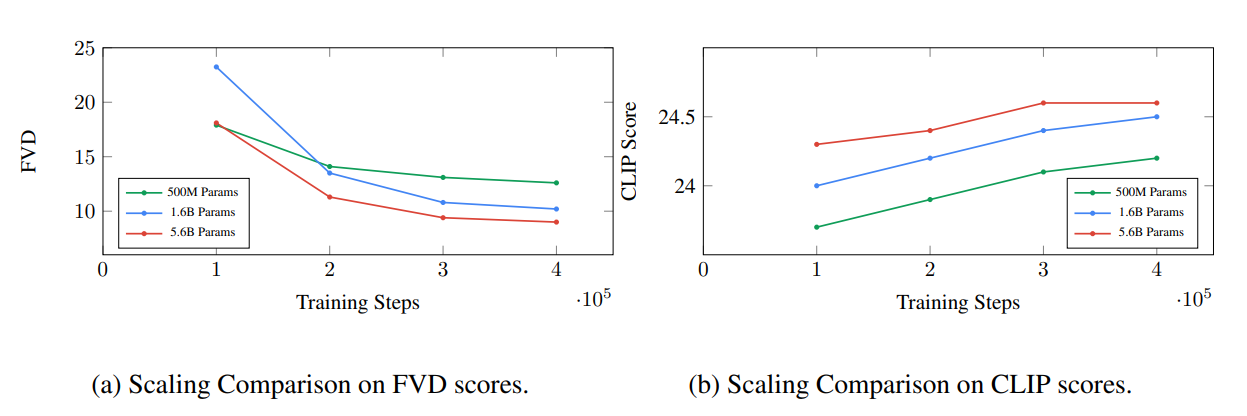
\includegraphics[width=1\textwidth]{images/imagen_video/scaling.png}
    \caption{Imagen-Video scaling results on video U-Net. The more parameters the model has, the better the FVD and CLIP scores.}
    \label{fig:imagen_video_scaling}
\end{figure}

\textbf{Scaling}: In figure \ref{fig:imagen_video_scaling} we can see the scaling comparison between different Imagen-Video models. \textbf{This result contradicts the findings of Imagen} \cite{imagen} paper; they found that increasing the U-Net size doesn't scale the sample quality as much as increasing the text encoder size. They conclude that video modeling task for which the performance is not yet saturated at current model sizes \footnote{This finding could hint that transformers, which benefit from scaling, could provide the necessary scaling capabilities that video modeling task demands.}.

\begin{figure}
    \centering
    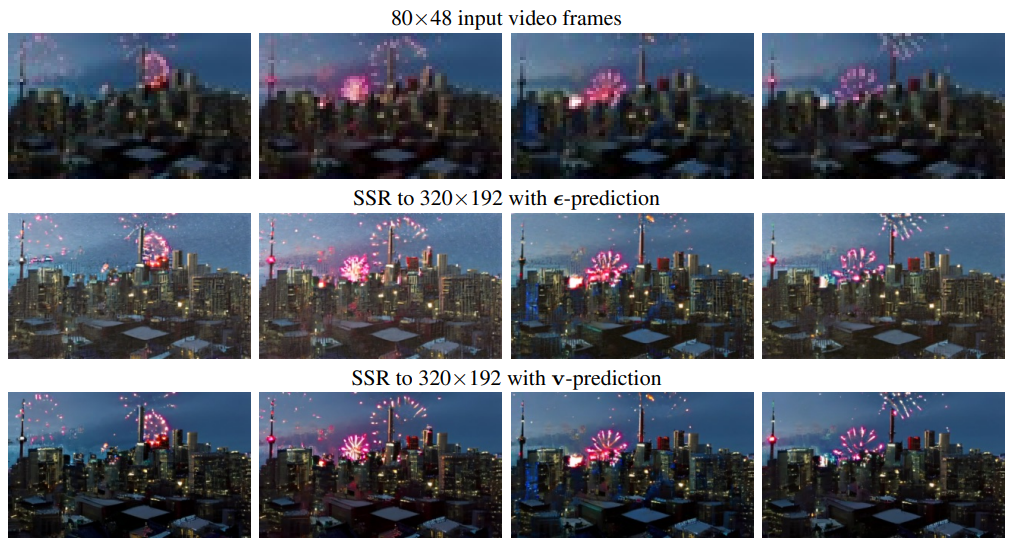
\includegraphics[width=0.8\textwidth]{images/imagen_video/e_prediction_vs_v_prediction.png}
    \caption{$\epsilon$-prediction (middle row) v.s. v-prediction (bottom row). In $\epsilon$-prediction we see color shifts across frames, whereas v-prediction is more consistent.}
    \label{fig:imagen_video_epsilon_prediction_vs_v_prediction}
\end{figure}

\begin{figure}
    \centering
    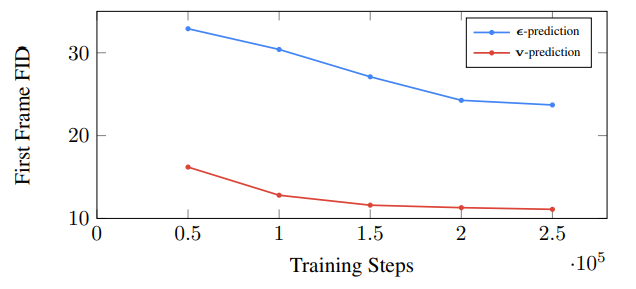
\includegraphics[width=0.6\textwidth]{images/imagen_video/e_prediction_vs_v_prediction_2.png}
    \caption{$\epsilon$-prediction v.s. v-prediction parameterization. v-prediction converges faster.}
\end{figure}

\textbf{$\epsilon$-prediction v.s. v-prediction}: They found that v-prediction is more effective than $\epsilon$-prediction for SSR models, figure \ref{fig:imagen_video_epsilon_prediction_vs_v_prediction}.

\begin{figure}
    \centering
    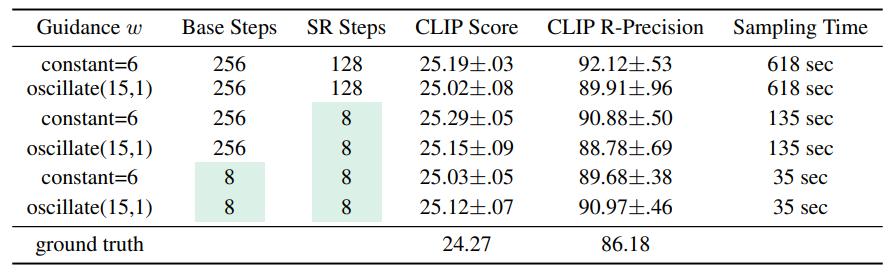
\includegraphics[width=0.8\textwidth]{images/imagen_video/experiments_table.png}
    \caption{Testing of fixed and oscillating guidance weight, distillation of base and SR models and evaluating each pipeline on CLIP score and sampling time. Distilling the pipeline results in significantly faster sampling time, while oscillating guidance weight improves the CLIP score a little.}
    \label{fig:imagen_video_experiments_table}
\end{figure}

\textbf{Distillation}: They found that distillation provides a good trade-off between sampling time and quality (figure \ref{fig:imagen_video_experiments_table}). \textbf{Distilled model is 18x times faster} in sampling, without significant degradation in perceptual quality. The distilled model is \textbf{also 36x more efficient} in terms of compute cost (FLOPs). 